%S09 cp7t; S07 cp6f

\begin{problem}
A \emph{5-path} communication network is shown below.  From this, it's
easy to see what an $n$-path network would be.  Fill in the table of
properties below, and be prepared to justify your answers.

\begin{center}
\begin{tabular}{ccc}
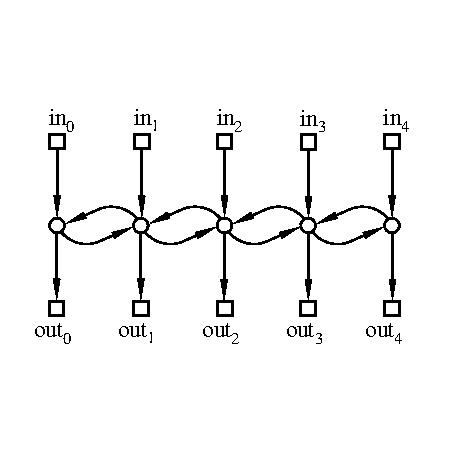
\includegraphics[height=1.5in]{line-nw}\\
% & & 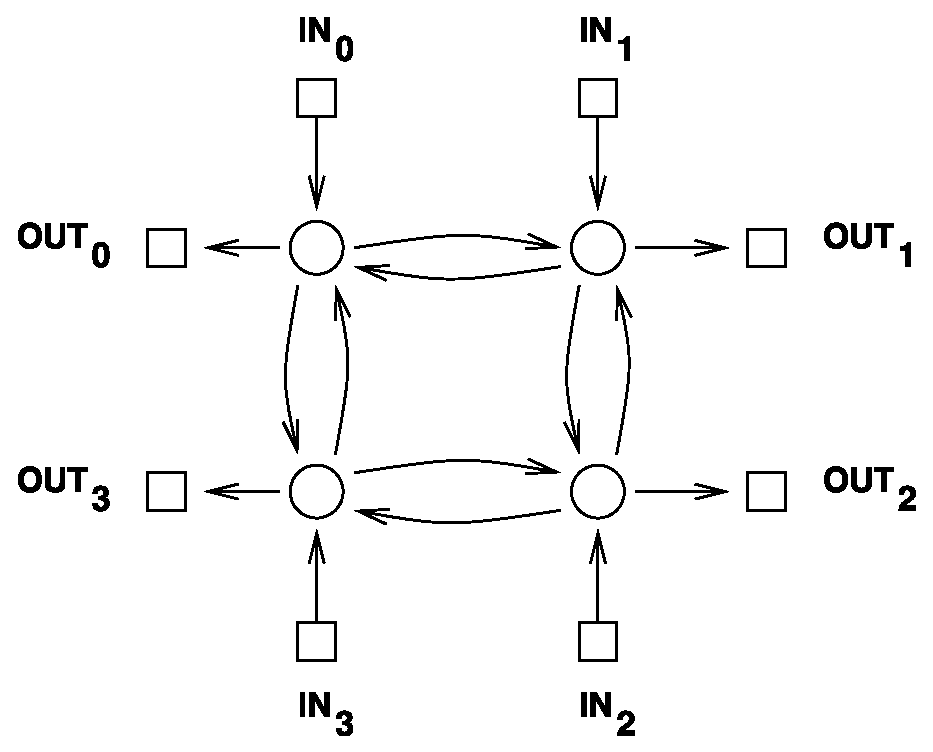
\includegraphics[height=2in]{cycle4} \\
\textbf{5-Path}% & \qquad & \textbf{4-Cycle}
\end{tabular}
\end{center}

{\large
\[
\begin{array}{c|c|c|c|c}
\text{network} &
\text{\# switches} &
\text{switch size} &
\text{diameter} &
\text{max congestion} \\ \hline
\text{5-path} &
\insolutions{5} &
\insolutions{3 \times 3} &
\insolutions{6} &
\insolutions{5} \\ \hline
\text{$n$-path} &
\insolutions{n} &
\insolutions{3 \times 3} &
\insolutions{n+1} &
\insolutions{n}
\end{array}
\]
}

\begin{solution}
The congestion of the $n$-path is at least $n$, because every
path must contain the central switch when $\pi(i) = n- 1 - i$.  The congestion
is at most $n$, because there are only $n$ simple paths in total.  The longest
path is from input 0 to output $n-1$ of length $n+1$, so this is the
diameter.
\end{solution}

\iffalse
The congestion of the 4-cycle is at least 3.  Consider the permutation
routing problem in which each input sends a packet to the diagonally
opposite output: $\pi(0) = 2$, $\pi(1) = 3$, $\pi(2) = 0$, $\pi(3) =
1$.  Packets 0 and 2 must pass through the switches on the upper left
and lower right in order to access the appropriate input and output
terminals.  Packets 1 must pass through one of these switches as well,
so at least three packets pass through either the upper-left switch or
the lower-left switch.

The congestion of the 4-cycle is at most 3.  Suppose we route each
packet by the shortest path and break ties by routing clockwise around
the cycle.  Now consider any particular switch, say the one in the
upper right.  At worst, this switch sees three packets: the one from
input 1, the one destined for output 1, and one passing through from
input 0 to output 2.  By symmetry, every switch sees at most 3 packets.}
\fi

\iffalse

\ppart Now consider the $n$-path and $2k$-cycle networks, and again fill in the
table below. (The $2k$-cycle is a $k \times k$ rectangular arrangement
with $k$ inputs on the top and bottom sides of the rectangle, and $k$
outputs on the left and right sides.)


{\large
\[
\begin{array}{c|c|c|c|c}
\text{network} &
\text{\# switches} &
\text{switch size} &
\text{diameter} &
\text{max congestion} \\ \hline
\text{$n$-path} &
\insolutions{n} &
\insolutions{3 \times 3} &
\insolutions{n+1} &
\insolutions{n} \\ \hline
\text{$2k$-cycle} &
\insolutions{4(k-1)} &
\insolutions{ 3 \times 3, 2\times 3, 3 \times 2 } &
\insolutions{2(k-1)+2 = 2k} &
\insolutions{k+1}
\end{array}
\]
}

\begin{solution}
TBA

\begin{figure}[h]
\graphic[height=3in]{2kCycle}
\end{figure}

\end{solution}

\end{problem}


\begin{problem}
A \emph{binary-tree network} has $n$ inputs and $n$ outputs, where $n$ is
a power of 2.  Each input is connected to the root of a binary tree with
$n/2$ leaves and with edges pointing away from the root.  Likewise, each
output is connected to the root of a binary tree with $n/2$ leaves and
with edges pointing toward the root.

Two edges point from each leaf of an input tree, and each of these edges
points to a leaf of an output tree.  The matching of leaf edges is
arranged so that for every input and output tree, there is an edge from a
leaf of the input tree to a leaf of the output tree, and every output tree
leaf has exactly two edges pointing to it.

\bparts
\ppart Draw such a binary-tree net for $n=4$.

\begin{solution}

\begin{figure}[h]
\graphic[height=3in]{binnet}
\end{figure}

\end{solution}


\ppart Fill in the table, and explain your entries.

{\large
\[
\begin{array}{c|c|c|c}
\text{\# switches} &
\text{switch size} &
\text{diameter} &
\text{max congestion} \\ \hline
&&&\\ \hline
\end{array}
\]
}

\begin{solution}

{\large
\[
\begin{array}{c|c|c|c}
\text{\# switches} &
\text{switch size} &
\text{diameter} &
\text{max congestion} \\ \hline
2n(n-1)& 1 \times 2, 2 \times 1 & 1+ 2\log n & 1\\ \hline
\end{array}
\]

\end{solution}

\iffalse
\begin{align*}
\text{\# switches } & = 2n(n-1)\\
\text{switch size} & = 1 \times 2, 2 \times 1\\
\text{diameter} & =  1+ 2\log n\\
\text{max congestion} & =1
\end{align*}
\fi

These formulas were gotten as follows: a binary tree with $n/2$ leaves has
$n-1$ nodes (switches), and there are $2n$ trees.

Each node of an input tree has one edge in and two out; the opposite
for nodes of output trees.

The distance from any input to any output is 1 from input to tree root,
$(\log n)-1$ from root to leaf, 1 from input leaf to output leaf, $(\log
n)-1$ from output leaf to output root, and 1 to output, for a total of $1+
2\log n$.

The path from any input to any output is unique, and paths from two inputs
to different outputs don't overlap, so at most one packet goes through any
switch.}

\eparts

\end{problem}


%%%%%%%%%%%%%%%%%%%%%%%%%%%%%%%%%%%%%%%%%%%%%%%%%%%%%%%%%%%%%%%%%%%%%%%%%%%%%%%

%\instatements{\newpage}

\begin{problem}
The Bene\u{s} network has a max congestion of 1; that is, every
permutation can be routed in such a way that a single packet passes
through each switch.  Let's work through an example.  A Bene\u{s} network
of size $N = 8$ is attached.

\bparts

\ppart Within the Bene\u{s} network of size $N = 8$, there are two
subnetworks of size $N = 4$.  Put boxes around these.  Hereafter,
we'll refer to these as the \textit{upper} and \textit{lower}
subnetworks.

\begin{solution}

\begin{figure}[h]
\graphic[height=2in]{benes-decomp}
\end{figure}

\end{solution}

\ppart Now consider the following permutation routing problem:
%
\begin{align*}
\pi(0) & = 3 & \pi(4) & = 2 \\
\pi(1) & = 1 & \pi(5) & = 0 \\
\pi(2) & = 6 & \pi(6) & = 7 \\
\pi(3) & = 5 & \pi(7) & = 4
\end{align*}
%
Each packet must be routed through either the upper subnetwork or the
lower subnetwork.  Construct a graph with vertices 0, 1, \ldots, 7 and
draw a \textit{dashed} edge between each pair of packets that can not
go through the same subnetwork because a collision would occur in the
second column of switches.

\begin{solution}

\begin{figure}[h]
\grahic[height=2in]{rec-const1}
\end{figure}

\end{solution}

\ppart Add a \textit{solid} edge in your graph between each pair of
packets that can not go through the same subnetwork because a
collision would occur in the next-to-last column of switches.

\begin{solution}

\begin{figure}[h]
\graphic[height=2in]{rec-const2}
\end{figure}

\end{solution}

\ppart Color the vertices of your graph red and blue so that adjacent
vertices get different colors.  Why must this be possible, regardless
of the permutation $\pi$?

\begin{solution}

This must be possible, because edges in a cycle are
alternately dashed and solid.  Thus, every cycle has even length,
which implies that the graph is bipartite or, equivalently,
2-colorable.

\begin{figure}[h]
\graphic[height=2in]{rec-const3}
\end{figure}

\end{solution}

\ppart Suppose that red vertices correspond to packets routed through
the upper subnetwork and blue vertices correspond to packets routed
through the lower subnetwork.  On the attached copy of the Bene\u{s}
network, highlight the first and last edge traversed by each packet.

\begin{solution}

\begin{figure}[h]
\graphic[height=3in]{rec-benes1}
\end{figure}

\end{solution}

\ppart All that remains is to route packets through the upper and
lower subnetworks.  One way to do this is by applying the procedure
described above recursively on each subnetwork.  However, since the
remaining problems are small, see if you can complete all the paths 
on your own.

\begin{solution}

\begin{figure}[h]
\graphic[height=3in]{rec-benes2}
\end{figure}

\end{solution}

\eparts
\end{problem}

%======================================


\iffalse

One prob on nets is enough.  To use this one, the terminology re
latency and max-congestion needs to be rewritten to match this term's
notes.  So I'm cutting it.  --ARM
\fi

%commented out of S09 ps7
\begin{center}
\begin{tabular}{ccc}
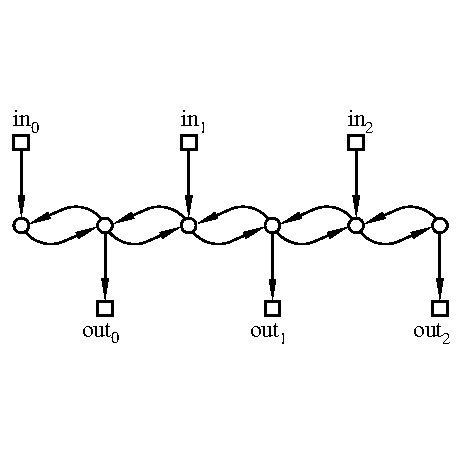
\includegraphics[height=2.0in]{MQ_oct31_network}\\
\end{tabular}
\end{center}

\begin{problem}[4] For the above communication network:

\bparts

\ppart[1] What is the max congestion? \hfill \examrule{0.5in}

\begin{solution}
The congestion of the network is at least 3,
  because every path must contain the central switches when $\pi(i) = 2 -
  i$.  The congestion is at most 3, because there are only 3 simple paths
  in total.
\end{solution}

\ppart[1] Give an input/output permutation, $\pi_0$, that forces maximum
  congestion:

\hfill $\pi_0(0) =$ \brule{0.4in}  \qquad $\pi_0(1) =$ \brule{0.4in}
\qquad $\pi_0(2) =$ \brule{0.4in}

\begin{solution}
The permutation $\pi_0$ is the same as the one specified in
  part (a)---$\pi_0(i) = 2-i$.  All three paths contain the central
  switch. 
\end{solution}

\ppart[1]\label{minpi} Give an input/output permutation, $\pi_1$, that
allows \emph{minimum} congestion:

\hfill $\pi_1(0) =$ \brule{0.4in}  \qquad $\pi_1(1) =$ \brule{0.4in}
\qquad $\pi_1(2) =$ \brule{0.4in}

\begin{solution}
The permutation is $\pi_1(i) = i$---each switch has only
one path going through it, so the congestion is $1$.
\end{solution}


\ppart[1] What is the latency for the permutation $\pi_1$? (If you could not find $\pi_1$, j
ust choose a permutation and find its latency.)
\hfill\examrule{0.5in}

\begin{solution}
\textbf{3}.  This is the latency of
  the (unique) shortest path routing for the permutation in
  part~\eqref{minpi}.  No smaller latency is possible since the minimum
  distance from any input to any output is 3.
\end{solution}
\eparts



{\large
\[
\begin{array}{c|c|c}
%\text{\# switches} &
%\text{switch size} &
\text{diameter} &
\text{latency} &
\text{max congestion} \\ \hline
%\insolutions{6} &
%\insolutions{2 \times 3, 3 \times 2} &
\insolutions{7} &
\insolutions{7} &
\insolutions{3}
\end{array}
\]
}



  The diameter of a communicaion net is the largest distance from an input
  to an output.  In this example, the largest distance is from input 0 to
  output 2 of length 7, so the diameter is 7.

  Latency depends on how packets are routed.  If you choose a shortest
  path routing, then the worst I/O pattern (permutation) will be the one
  that maps the maximum distance input to output, so the latency will
  equal the diameter.

  However, a shortest-path routing may be pretty congested, so we're
  usually more interested in the worst latency among the
  minimum-congestion routings.  But in this example, the shortest path
  routing is also the minimum congestion routing, so the latency is any
  case equals the diameter, namely 7.
  
\end{problem}


%S09 ps7

\begin{problem}
Louis Reasoner figures that, wonderful as the Bene\u{s} network may be, the
butterfly network has a few advantages, namely: fewer switches, smaller
diameter, and an easy way to route packets through it.  So Louis designs an
$N$-input/output network he modestly calls a \textit{Reasoner-net} with the
aim of combining the best features of both the butterfly and Bene\u{s} nets:
\begin{quote}
The $i$th input switch in a Reasoner-net connects to two switches, $a_i$
and $b_i$, and likewise, the $j$th output switch has two switches, $y_j$
and $z_j$, connected to it.  Then the Reasoner-net has an $N$-input
Bene\u{s} network connected using the $a_i$ switches as input switches and
the $y_j$ switches as its output switches.  The Reasoner-net also has an
$N$-input butterfly net connected using the $b_i$ switches as inputs and<
the $z_j$ switches as outputs.
\end{quote}

In the Reasoner-net a minimum latency routing does not have minimum
congestion.  The \textit{latency for min-congestion} (LMC) of a net is the
best bound on latency achievable using routings that minimize congestion.
Likewise, the \textit{congestion for min-latency} (CML) is the best bound
on congestion achievable using routings that minimize latency.

Fill in the following chart for the Reasoner-net and briefly explain your
answers.

\[
\begin{array}{|c|c|c|c|c|c|}
\textbf{diameter} &
\textbf{switch size(s)} &
\textbf{\# switches} &
\textbf{congestion} &
\textbf{LMC} &
\textbf{CML}\\
\hline
&&&&&\\
\hline
\end{array}
\]

\begin{solution}

\[
\begin{array}{|c|c|c|c|c|c|}
\textbf{diameter} &
\textbf{switch size(s)} &
\textbf{\# switches} &
\textbf{congestion} &
\textbf{LMC}&
\textbf{CML}\\
\hline \log N + 4 & 2 \times 2 & 3N (\log N + 1) & 1 & 2 \log N +
3 &
\sqrt{N}\\
\hline
\end{array}
\]

or

\[
\begin{array}{|c|c|c|c|c|c|}
\textbf{diameter} & \textbf{switch size(s)} & \textbf{\# switches}
& \textbf{congestion} & \textbf{LMC}&
\textbf{CML}\\
\hline \log N + 2 & 2 \times 2 & 3N (\log N + 1) & 1 & 2 \log N +1
&
\sqrt{N}\\
\hline
\end{array}
\]

%REVISE wrt to current notes --ARM

There are two possible answers for the diameter, because in lecture the
special ``square'' input/output switches were not used (they mess up the
recursive definitions).  To match the Notes, these switches have to be
added after the recursion, increasing the diameter by 2.  So the first
answer corresponds to the lecture notes, and the second one corresponds to
the slides.

The diameter of a Reasoner-net is 2 plus the smaller of the
diameters of its Bene\u{s} component, $2 \log N + 1$ or $2\log
N-1$, and its butterfly component, $\log N +2$ or $\log N$.

The number of switches is the number of input and output switches in the
Reasoner-net, namely, $2N$, plus the number of switches in its butterfly
component, $N (\log N + 1)$, and its Bene\u{s} component, $2N \log N$.

The congestion is the congestion of the better of the two component nets.

The LMC for the butterfly net equals its diameter, and likewise for the LMC
of the Bene\u{s} net.  So the LMC of the Reasoner-net is 2 plus the LMC of
the routing through the component with minimum congestion, namely, 2 plus
the diameter of the Bene\u{s} net.

The CML equals the congestion of the routing through the component
with minimum latency, namely, the congestion of butterfly net.
\end{solution}

\end{problem}
